\chapter{Theoretischer Hintergrund}

\section{Lerntypeneinteilung nach \citeauthor{gagnebedingung} (\citedate{gagnebedingung})}

Gagné unterteilt seine Formen des Lernens hierarchisch. Somit setzen die nachfolgenden Lernarten die vorhergehenden Lernarten voraus. Generell wird in zwei Teile unterteilt: 


\begin{itemize}
\item (A) Grundformen des Lernens: Assoziationen und Ketten 
    \begin{itemize}
        \item (A.1) Signallernen
        \item (A.2) Reiz-Reaktions-Lernen
        \item (A.3) Kettenbildung
        \item (A.4) Sprachliche Assoziation
    \end{itemize}
\item (B) Intellektuelle Fähigkeiten
    \begin{itemize}
        \item (B.1) Diskriminationslernen
        \item (B.2) Begriffslernen
        \item (B.3) Regellernen 
        \item (B.4) Problemlösen
    \end{itemize}
\end{itemize}

\subsection[]{(A.1) Signallernen (\citeauthor{pawlow1977klassische} `s (\citedate{pawlow1977klassische}) "klassische" Konditionierungslehre)}

Man versucht mit einem Reiz eine dadurch bedingte Reaktion hervorzurufen. Eines der bekanntesten pädagogischen Phänomene dazu, ist der "Pawlowsche Hund". Hierbei wird immer, bevor ein Hund Futter bekommt eine Glocke geschlagen. Nach einigen Durchgängen ertönt nur noch das Klingen der Glocke, was den Speichelfluss des Hundes anreizt, ohne dass er Futter bekommt. Somit können einfache Reize ( z.B Ton), bestimmte Reaktionen (z.B Speichelfluss) auslösen, welche nicht reflexartig angeboren, sondern antrainiert wurden.

\subsection[]{(A.2) Reiz-Reaktions-Lernen (Trial and Error Prinzip, Lernen durch Verstärkung)}

Der Lernende versucht etwas so lange auf verschiedene Art und Weise, bis es klappt und merkt sich anschließend wie es zu Erfolg führte. 
Beispiel: Jemand ist sich bei der letzten Nummer seines Fahrradschlosses unsicher. Er probiert deswegen  alle Möglichkeiten von 0 – 9 aus und merkt sich bei welcher Zahl das Schloss aufgegangen ist. Hierbei erfährt der Lernende eine Verstärkung, weil er danach mehr kann als davor ( in unserem Beispiel: Schloss öffnen) und dies nur durch einfaches Ausprobieren geschafft hat.

\subsection[]{(A.3) Kettenbildung (Lernen von Abläufen)}

In diesem Fall werden längere Reiz-Reaktions-Ketten gebildet. Hierbei sind alle Formen von Algorithmen oder Verfahren eingeschlossen. Beispiele: Kochen, Telefonieren, oder auch Klammern im Mathematikunterricht auflösen. Diese Ketten können meist verstanden und durchgeführt werden, ohne einen tieferen Sinn des einzelnen Verfahrens verstanden zu haben. In der Schule kann diese Lernart zu Problemen führen, da die \gls{SuS} kein Verständnis für die Zusammenhänge haben müssen, lediglich ihre Algorithmen durchgehen können. Dies kann in Aufgaben mit höherem Abstraktionsgrad zu Problemen führen, wenn das Schema nicht mehr ohne Weiteres anwendbar ist.

\subsection[]{(A.4) Sprachliche Assoziation (verbales auswendig Lernen)}

Hierbei werden bestimmte Definitionen, Gedichte oder Ähnliches so lange wiederholt, bis sie auswendig vom Lernenden vorgetragen werden können. Somit findet eine Verkettung oder auch Assoziation von einfachen Objekten - in unserem Fall Wörtern - statt. Es werden ebenso, wie in den anderen Grundformen, lediglich die Verknüpfungen der Wörter geschaffen und kein Verständnis dabei erzeugt. 

\subsection[]{(B.1) Diskriminationslernen (Unterscheidungslernen)}

In diesem Fall soll der Lernende verschiedene Gegenstände und Merkmale als verschieden auffassen können. Beispiele: Ein bestimmtes Passwort passt nur zu einem bestimmten Account. Oder: Nicht jedes Fahrrad sieht gleich aus. Es gibt Rennräder, Stadträder, Lastenräder und viele mehr. Der Lernende soll hierbei ein besseres Verständnis für Begriffe entwickeln, indem er lernt, diese zu differenzieren.

\begin{figure}[!ht]
\noindent\hspace{0.5mm}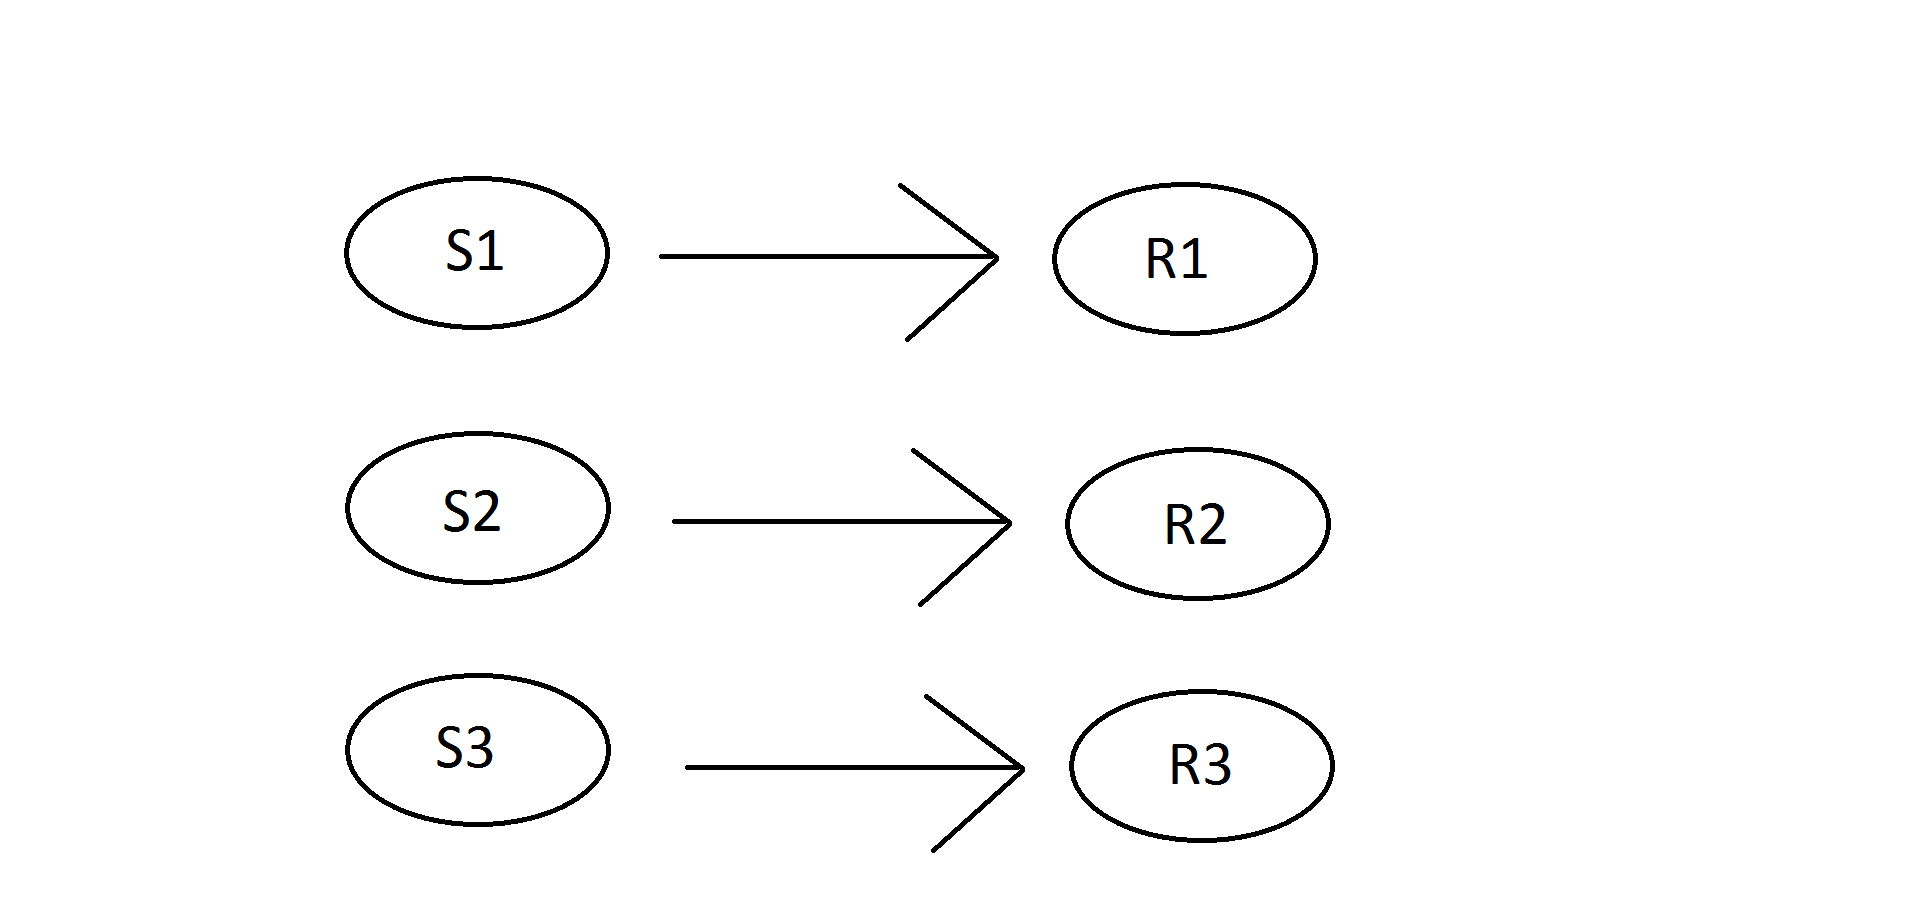
\includegraphics[width=12cm]{./Ressourcen/Begriffslernen.png}
\caption{Diskriminationslernen, Zech}
\end{figure}

\subsection[]{(B.2) Begriffslernen (Gemeinsamkeiten finden)}

Bei diesem Typ soll genau der konträre Weg zum Diskriminationslernen begangen werden. Es sollen unterschiedliche Objekte, als \textit{gleich} zusammengefasst werden können. 
Beispiele: ein Rechteck und ein Quadrat sind beides Vierecke, oder ein Audi Q7 und ein BMW X5 sind SUVs. Somit können bessere Verbindungen zwischen Lerngegenständen hergestellt und sich auf allgemeine Details zurückgezogen werden (z.B Winkelsumme Viereck sind 360 Grad, Auto hat einen Motor).


\begin{figure}[!ht]
\noindent\hspace{0.5mm}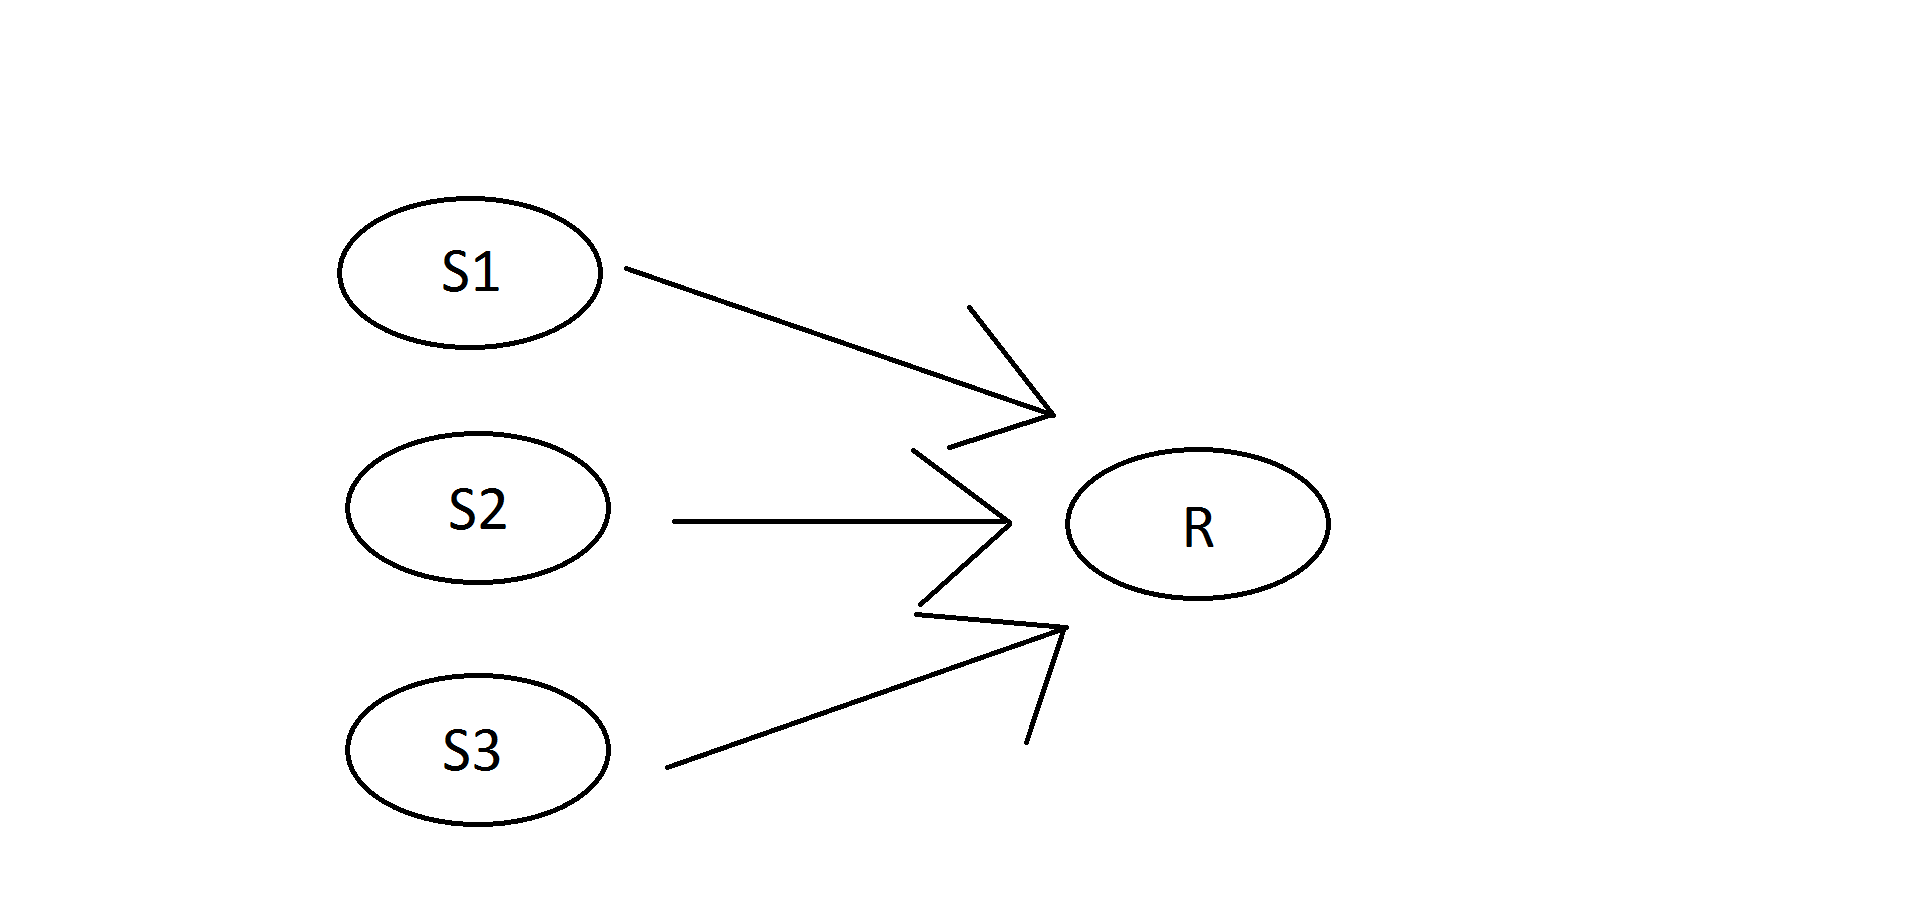
\includegraphics[width=12cm]{./Ressourcen/Diskrimination.png}
\caption{Begriffslernen, Zech}
\end{figure}

\subsection[]{(B.3) Regellernen (Regeln für Anwendungsbereiche lernen)}

Beim Regellernen ist nicht nur das einfache auswendig Lernen von Regeln oder Ähnlichem gemeint, sondern das damit verbundene Verständnis. Somit kann also der Kontext des Satzes des Pythagoras aufgefasst werden: Zum einen ist die Formel $a^2$ + $b^2$ = $c^2$ im aktiven Wissen vorhanden, zum anderen sind auch die Anwendung und die Bedingungen der Formel verständlich.

\subsection[]{(B.4) Problemlösen (Aufgaben mit eigenen Überlegungen lösen)}

Dies ist der nächste Schritt vom Regellernen, da hierbei Regeln verstanden sein müssen und diese kombiniert in einer Aufgabe angewendet werden können. Somit gehört in der Gagnéschen Hierarchie der Problemlöser zur höchsten Ordnung, da seine Kompetenzen die Kompetenzen der vorhergehenden Typen beinhalten.

\section{Lerntypeneinteilung nach \citeauthor{zech1983grundkurs} (\citedate{zech1983grundkurs})}

Die Lerntypen von Gagné werden in der Einteilung nach Zech aufgegriffen, zusammengefasst und erweitert, um neue Lerntypen zu definieren. Ebenso betrachtet er die Lerntypen hauptsächlich im Kontext der Mathematik und nicht auf alle Lerngegenstände bezogen. Zech unterteilt seine Lerntypen nicht mehr hierarchisch und gibt klare Lernbediengungen für den jeweiligen Lerntypen an. Es werden die folgenden fünf Typen betrachtet:

\subsection[]{Assoziatives Lernen}

In dieser Unterteilung sind die im kognitiven Bereich beschränkten Grundformen des Lernens (Teil A) nach Gagné zusammengefasst. Somit werden bei diesem Typ " kürzere oder längere Reiz-Reaktions-Verbindungen (Automatismen)\grqq  aufgebaut und jene hauptsächlich auswendig gelernt. Dies kann im mathematischen Sinne, als das Anwenden von bekannten Regeln auf einfache Aufgabentypen verstanden werden. Außerdem bezieht sich dieser Typ neben der Abstammung von den Grundformen (A), mehr auf texttuelle als auf bildliche Teile von Aufgaben.
Die Lernbedingung dieses Types ist: häufige Wiederholung. 
Anhand dessen entsteht in der Unterteilung des Versuchaufbaus dieser Arbeit die Gruppierung \gls{Gr1}, welche sich dadurch auszeichnet, dass das heuristische Beispiel sehr häufig wiederholt gelesen wird und somit die Fokussierung auf den Text im Vordergrund steht. 


\subsection[]{Diskriminationslernen}

Er wird zu großen Teilen aus dem Typ von B.1 abgeleitet, wie der Name auch schon vermuten lässt. Hierbei wird aber nochmals verdeutlicht, dass das Diskriminationslernen als Voraussetzung zum Begriffslernen stehen muss, da erst Objekte unter einem Begriff zusammengefasst sein müssen, bevor sie als unterschiedlich erkannt werden können.
Lernbedingungen: Unterschiede hervorheben (zum Beispiel mit bunter Kreide), Kontiguität (Angrenzung, Berührung) (aus \cite{DudenKontiguitaet}).
Dieser Lerntyp ist in der gegebenen Studie schwer von den anderen Typen zu unterscheiden, da sich die Aufgabenstellung nicht explizit mit Diskrimination befasst, sondern mit dem Lösen mathematischer Probleme. Somit wird dieser Lerntyp in der Studie nicht weiter behandelt.

\subsection[]{Lernen mathematischer Begriffe}

Dieser Typ baut sich auch auf dem Lerntyp B.2 Begriffslernen auf. Zunächst werden die Begriffe unterteilt in: Eigenschaftsbegriffe, Relationsbegriffe und zusammengesetzte Begriffe. Eigenschaftsbegriffe beschreiben Merkmale oder Eigenschaften eines Objektes. Relationsbegriffe beschreiben eine Relation zwischen verschiedenen Objekten, wie z.B A hat mehr Kanten wie B. Zusammengesetzte Begriffe werden aus einer Kombination von ursprünglichen Begriffen definiert z.B \textit {eine Teilmenge des euklidischen Raums R n heißt kompakt, wenn sie abgeschlossen und beschränkt ist}.\\ Diese Begriffe sollen durch die Zusammensetzung mehrerer bekannter Begriffe verstanden werden. Dieser Lerntyp baut auf B.3 Regellernen auf. Die Begriffe gehen durch Abstraktion aus der Erfahrungswelt hervor.
Lernbedingungen: relevante Merkmale hervorheben, mehrere Beispiele (irrelevante Merkmale variieren), Gegenbeispiele.
Leider sind die gegebenen Lernbedingungen anhand einer Eyetracking-Studie, bei der nichts markiert wird, oder \gls{dPodP} weder Beispiele noch Gegenbeispiele anbringen kann, nicht auszuwerten. Aus diesem Grund wurde dieser Lerntyp in der Studie ebenfalls nicht weiter behandelt. 

\subsection[]{Lösen mathematischer Probleme}

Unter diesem Lerntyp wird ein Verinnerlichen mathematischer Zusammenhänge verstanden. Hierbei wird das Lernen heuristischer Regeln vorausgesetzt. Es müssen zuerst bestimmte allgemeine Strategien (z.B. Widerspruchsbeweis) aufgenommen werden, um anschließend eine Transferleistung zu vollbringen, wie es bei Aufgaben mit hohem Abstraktionsgrad vorausgesetzt wird. 
Lernbedingungen: Problemlösungsfähigkeiten (analysieren, vergleichen, Beziehungen herstellen uvm.) umsetzen und heuristische Regeln einzusetzen.
In Anlehnung an den Typ "Lösen mathematischer Probleme" wird in meiner Arbeit die Gruppierung \gls{Gr2} definiert, welche sich sehr stark auf die Bilder fokussiert, nachdem sie den Text das erste Mal aufgenommen hat.

\section{Lerntypeneinteilung nach \citeauthor{schrader2008lerntypen} (\citedate{schrader2008lerntypen})}

Wie bereits angedeutet, unterteilt Schrader seine Lerntypen eher in Anlehnung an allgemeine Persönlichkeitstypen: der Theoretiker, der Anwendungsorientierte, der Musterschüler, der Gleichgültige und der Unsichere. Hierbei wird nicht mehr auf alle Typen eingegangen, da sich viele in den Gruppierungen von Zech widerspiegeln und die Persönlichkeitstypen in vorliegender Studie nicht ermittelt sind. Somit wird nur auf die Gruppierung "der Unsichere" eingegangen.

Der \gls{Gr3} sucht Ursachen bei sich und zweifelt an seinen Fähigkeiten. Das Lernen aus Texten fällt diesem Typ schwer, da er dabei wenig systematisch vorgeht. Er lässt sich lieber etwas mehr Zeit, um die gegebene Aufgabenstellung zu bearbeiten.
Lerncharakteristik: Da ihm das Arbeiten mit Texten Schwierigkeiten bereitet, ist die Bearbeitungszeit länger als gewöhnlich und es werden sowohl Text-, als auch Bildbereiche häufiger als bei gewöhnlichen \gls{PuP} betrachtet. 

\section{Effekte graphischer Darstellungen}

Laut einer Studie von \citeauthor{mayer2005reliability} (\citedate{mayer2005reliability}) hat das Arbeitsgedächtnis zwei Kanäle zur Verarbeitung von Informationen. Einer der Kanäle verarbeitet Informationen von Wörtern, der andere von Bildern. Somit kann eine optimale Lernbedingung geschaffen werden, indem sowohl verständlicher Text als auch passend eingebundene Bilder dem Lernenden zu Verfügung gestellt werden. Laut \citeauthor{bockmannvalue} (\citedate{bockmannvalue}) lassen sich Bilder in drei unterschiedliche Typen unterteilen:
    
    \begin{itemize}
        \item Dekorative Bilder (decorative pictures), welche keine echten Informationen über das gegebene Problem zeigen. Z.B. eine Radfahrerin, wenn es in der Aufgabe über das Zurücklegen einer Strecke mit dem Rad geht.
        \item Repräsentative Bilder (representational pictures), welche Teile der gestellten Aufgabe veranschaulichen. Z.B. ein Drachenviereck, wenn die Aufgabe gestellt ist: den Flächeninhalt eines Drachenvierecks zu bestimmen. 
        \item Essenzielle Bilder (essential pictures), welche Informationen geben die für die Bearbeitung der Aufgabe essenziell sind. Z.B. bei der Berechnung einer Fläche eine Graphik, in der relevante Längen von Seiten eingetragen sind.
    \end{itemize}

In der Studie wurden 217 \gls{SuS} aus der 9. Jahrgangsstufe in Gruppen eingeteilt. Bei dem Versuch wurden die \gls{SuS} in drei Gruppen unterteilt, welche dieselbe Aufgabenstellung erhielten, jedoch die Bildtypen sich unterschieden. In der Aufgabe wird von den \gls{SuS} verlangt, den Abstand von einer Person zu ihrem Lenkdrachen mit Hilfe des Satzes des Pythagoras zu berechnen. Die Aufgabestellung sollte von den \gls{SuS} nicht bearbeitet, sondern lediglich Fragen hierzu beantwortet werden. 


Die erste Gruppe erhielt die Aufgabenstellung mit einem dekorativen Bild (ein einfaches Abbildung eines Lenkdrachens).


Die zweite Gruppe erhielt ein Bild, in dem die beschriebene Situation (Person mit Schnurverbindung zum Lenkdrachen) bildlich dargestellt wurde (repräsentativ).


Die dritte Gruppe hingegen erhielt dasselbe Bild wie die zweite Gruppe, zusätzlich mit Längenangaben (essenziell).


Es konnte gezeigt werden, dass dekorative Bilder den \gls{PuP} kaum eine Unterstützung in der Lösung der gestellten Aufgaben geben. Hingegen repräsentative einen positiven Effekt und essenzielle Bilder den besten Effekt bewirkten.

